\documentclass[tikz, convert={density=72,outext=.png, outfile=tlb_adress.png}]{standalone}

\usetikzlibrary{backgrounds}

\begin{document}

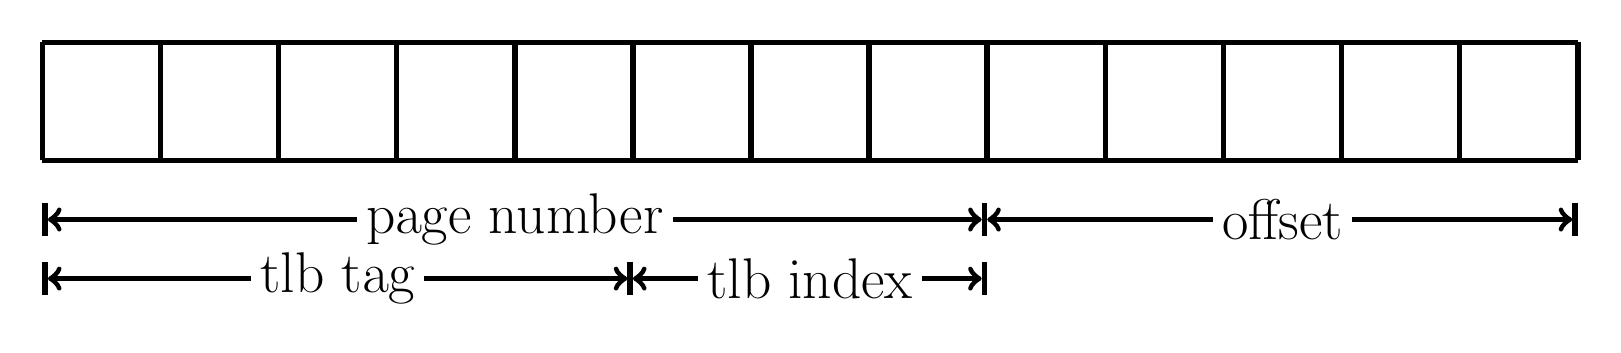
\begin{tikzpicture}[background rectangle/.style={fill=white}, show background rectangle]

  \edef\boxsize{1.5}
  \edef\boxnr{13}
  \tikzstyle{bits}=[line width=2pt]

  \foreach \i in {0,...,\boxnr}
    {
      \pgfmathsetmacro{\x}{\i * \boxsize}
      \draw[bits] (\x,0) -- (\x,\boxsize);
    }

  \pgfmathsetmacro{\boxend}{\boxnr * \boxsize}
  \draw[bits] (0,0) -- (\boxend,0);
  \draw[bits] (0,\boxsize) -- (\boxend,\boxsize);

  \pgfmathsetmacro{\pagenr}{8 * \boxsize}
  \pgfmathsetmacro{\tlbtag}{5 * \boxsize}

  % labels below
  \pgfmathsetmacro{\below}{-0.5 * \boxsize}
  \draw[bits] (0,\below) edge[|<->|] node[fill=white,font=\huge] {page number} (\pagenr,\below);
  \draw[bits] (\pagenr,\below) edge[<->|] node[fill=white, font=\huge] {offset} (\boxend,\below);
  
  % labels above
  \pgfmathsetmacro{\tlblayer}{-1 * \boxsize}
  \draw[bits] (0,\tlblayer) edge[|<->|] node[fill=white,font=\huge] {tlb tag} (\tlbtag,\tlblayer);
  \draw[bits] (\tlbtag,\tlblayer) edge[<->|] node[fill=white, font=\huge] {tlb index} (\pagenr,\tlblayer);
\end{tikzpicture}

\end{document}